.q%\epigraphfontsize{\small\itshape}
%\setlength\epigraphwidth{8cm}
%\setlength\epigraphrule{0pt}
%\epigraphfontsize{\small\itshape}
%\epigraph{If all mathematics disappeared today, physics would be set back exactly one week.}{---\textup{Richard Feynman}}


%\epigraph{There are two possible outcomes: If the result confirms the hypothesis, then you've made a measurement. If the result is contrary to the hypothesis, then you've made a discovery.}{---\textup{ Enrico Fermi}}

\section{Reconstruction of the SNO+}

\section{Reconstruction Algorithms for Position, Time and Energy of Events in SNO+}


\section{An Alternative Vertex Reconstruction Algorithm for SNO+}
A Multi-path Fitter (MPF) framework was developed by the University of Alberta group as an alternative reconstruction algorithm to the SNO+ official fitter. In this framework, fitters for SNO+ water phase (MP Water Fitter), wavelength shifter (MP WLS Fitter), partial-fill phase (MP Partial Fitter) and scintillator phase (MP Scint Fitter) were developed. In SNO+ water phase, the cavity and the AV are both filled with pure water. This is a relatively simple geometry. Therefore, we start with the MP Water Fitter to explain the reconstruction concepts.



First, the fitter throws a random vertex (uniformly distributing) inside the PSUP as a trial vertex. The Class Library for High Energy Physics (CLHEP) is used for creating pseudo-random numbers.

$rand0 = Uniform(0,1), rand1 = Uniform(-1,1)$  


  double ran0 = CLHEP::RandFlat::shoot( 0.0, 1.0 );
double ran1 = CLHEP::RandFlat::shoot( -1.0, 1.0 );
double ran2Pi = CLHEP::RandFlat::shoot( 0.0, 2.0*CLHEP::pi );
double t = CLHEP::RandFlat::shoot( 100.0, 300.0 );

double wl = CLHEP::RandFlat::shoot( 4000.0, 6000.0 );
double r = pow(ran0, 1.0/3.0) * fPSUPRadius; // mm
double costheta = ran1;
double sintheta = sqrt(1.0 - costheta*costheta);






The MP Water Fitter uses prompt light and assumes that photons propagate in straight lines (straight light paths) for likelihood calculations. Detailed situations, such as the reflection and lensing effects from different detector components are neglected. Figure~\ref{mpwdiagram} shows the reconstruction concepts for position and direction.


The MPW fitter currently fits for position, time and direction of a water phase event. The fitter uses prompt light and straight line paths for likelihood calculations. Then it utilizes the Multi-path Fitter to maximize the likelihood functions and find the best-fit values. The concept of this fitter is the same of the FTU fitter in SNO time.

\paragraph{MPW: Fitter Structure}

The MPW fitter consists of: 
\begin{itemize}
	\item Fitter Data : Includes physics constants, set-values and pdfs for the MPW fitter. These parameters are set in the MPW database.
	
	- Water reflection index (water\_RI, or n$_{water}$), used for group velocity ($v_g$ =c/n$_{water}$) calculation. 
	
	The MPW fitter currently uses one fixed number for n$_{water}$, rather than a function of wavelengths. The value of n$_{water}$ can be tuned to give the lowest biases of the fitted positions to the Monte Carlo and to give the lowest RMS of fitted results as well. But the effect of n$_{water}$ can also be corrected by the drive correction afterwards. Currently n$_{water}=1.38486$ is obtained by analyzing the time of flight from the \isotope[16]{N} central run-100934 data reconstructed by the MPW fitter. 
	
	- Constants for fit setting: Includes the fitter tolerance, the maximum iterations for the Multi-path Fitter to converge, time offset, radius cut for position vertex, fitting bin-width and steps.
	
	- Other physics constants: air reflection index (air\_RI), psup radius.
	
	- PMT response time (timing) pdf for the position reconstruction, as shown in \ref{MPW_timingPDF}. The pdf shown in red line is modified from the measured PMT response time distribution from SNO time and the late light response is forced to be de-weighted (black). The pdf is modified in [-100,-4] ns region to match the time residue spectrum obtained from %\isotope[16]{N} central run-100934 (blue).
	
	\begin{figure}[!htb]
		\centering
		%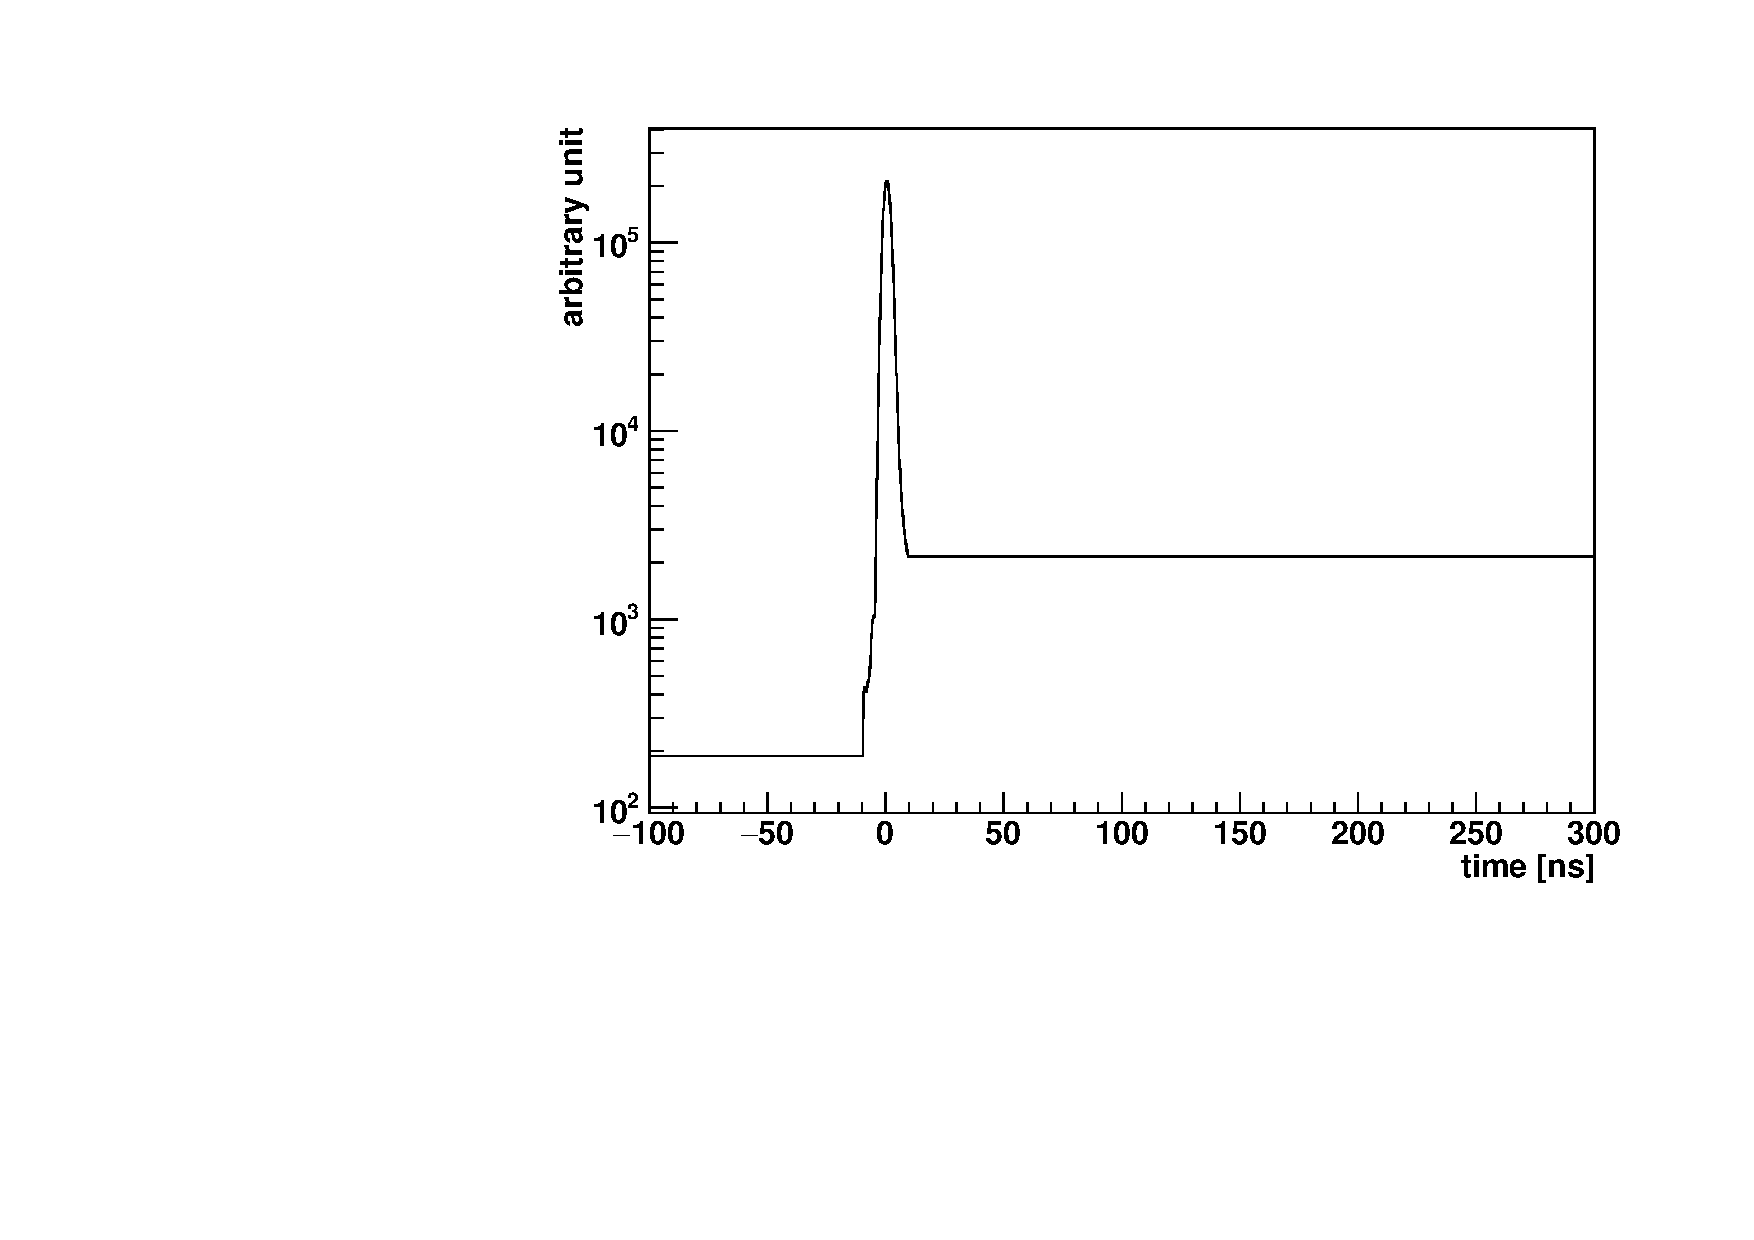
\includegraphics[width=10cm]{recon/MPW_timingPDF.pdf}
		\caption{PMT response time as the timing pdf.}
		\label{MPW_timingPDF}
	\end{figure}
	
	- PMT angular response pdf for the direction reconstruction, as shown in \ref{MPW_angularPDF}. It is taken from the Monte Carlo simulation of 5 MeV electrons traverse in the AV with one direction.
	
	\begin{figure}[!htb]
		\centering
		%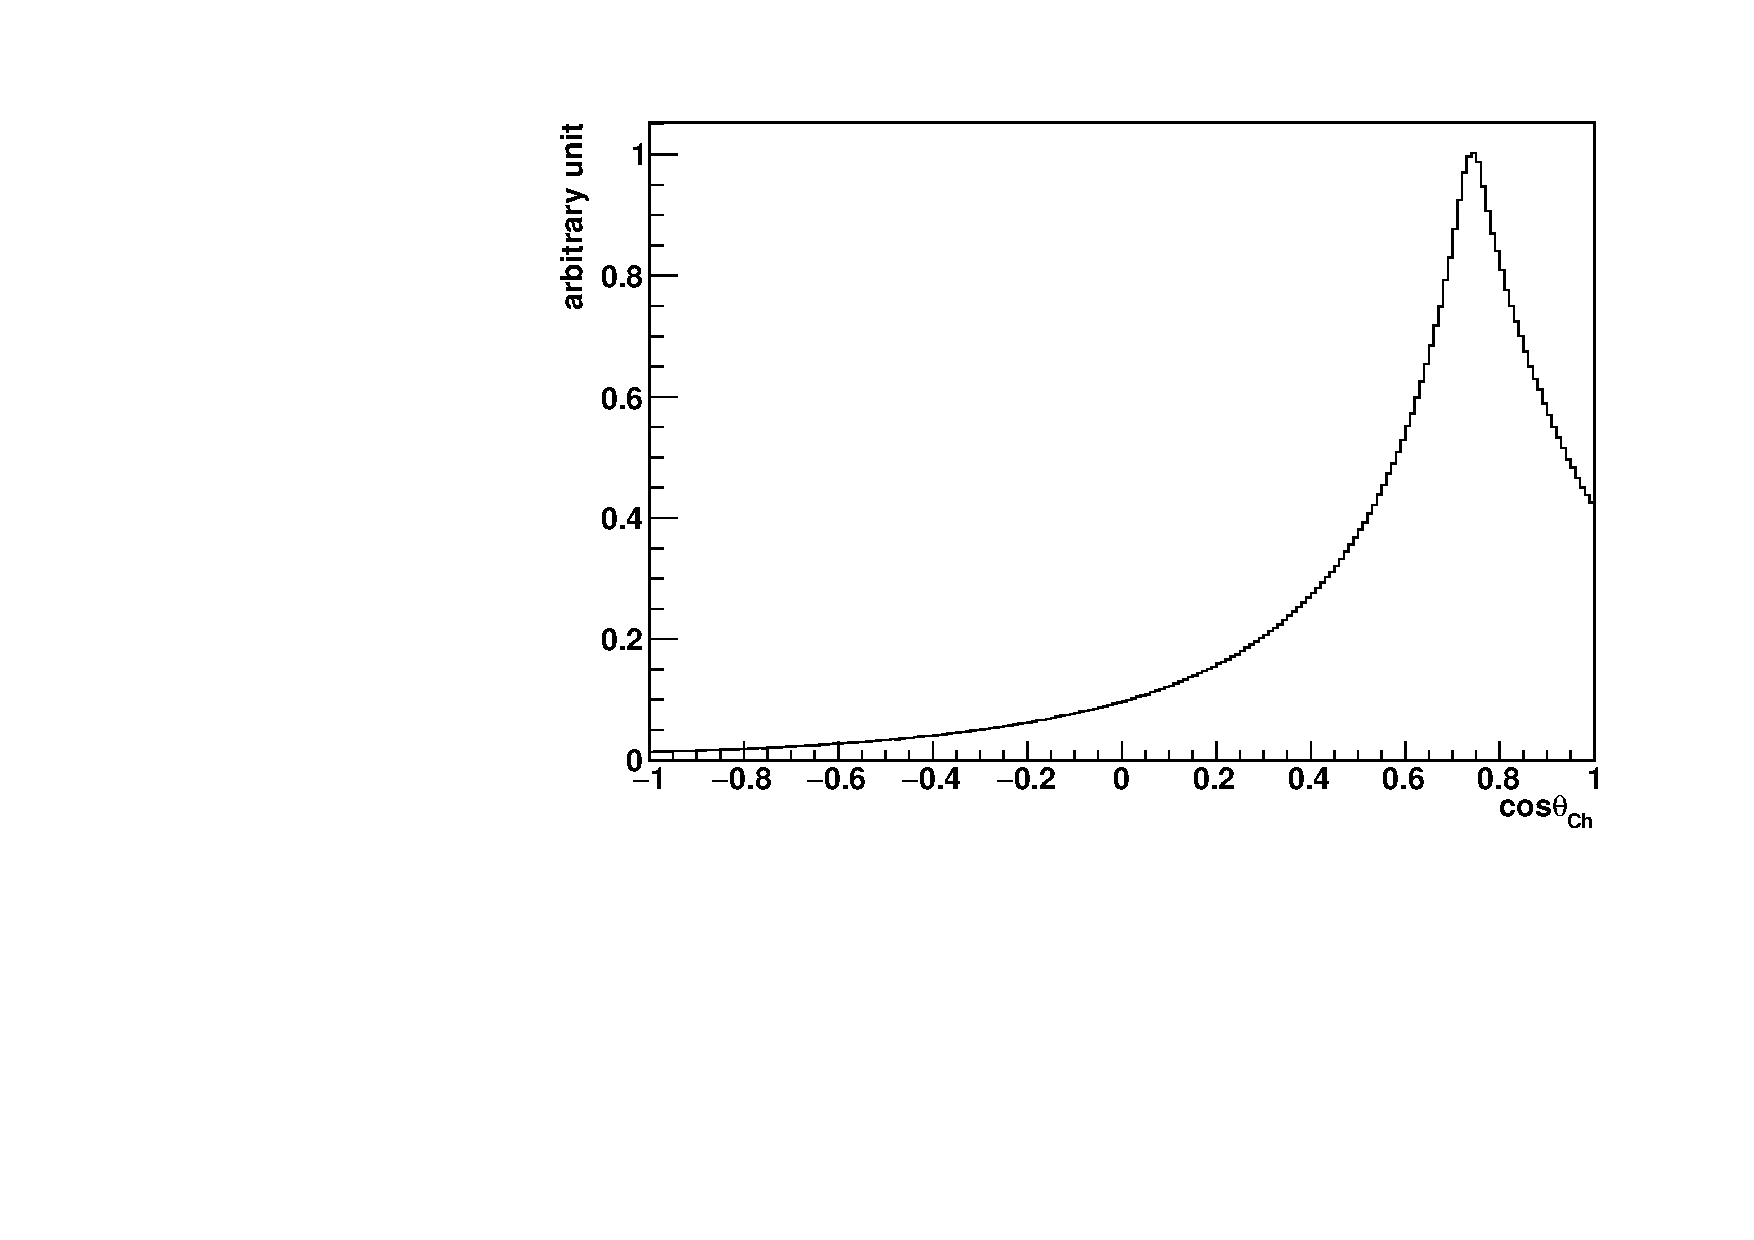
\includegraphics[width=10cm]{recon/MPW_angularPDF.pdf}
		\caption{PMT angular distribution as the angular response pdf.}
		\label{MPW_angularPDF}
	\end{figure}
	
	\item Fit the position, time and direction.
	
	- Likelihood Calculation Classes: Constructs likelihood functions, calculates likelihoods and their derivatives. For the MPW fitter, there are two classes: WaterPosition for position reconstruction and WaterDirection for direction reconstruction. The WaterPosition class tackles with 4 parameters (x,y,z,t) and the WaterDirection class tackles with 2 parameters ($\theta$,$\phi$). 
	
	- Multi-path Fitter: Processes the MPW fitter and finds the best-fit of the likelihood function. It is a general processor and is shared with the fitters using the Multi-path Fitter, including the MPW fitter, air-water (AW) fitter, wavelength-shifter (WLS) fitter and scint-water fitter (being developed). It processes a certain fitter by being assigned the fitter name in macro. It processes the fitter event by event: for every triggered event, it first calls PMT selectors (ModeCut or StraightTimeResidualCut) and sends the information of the reduced PMTs to a certain Likelihood Calculation Class for likelihood calculations. The Likelihood Calculation Class sends back the values of likelihoods and their derivatives, so the Multi-path Fitter does not care about how the likelihood functions are constructed and how the likelihoods and derivatives are calculated. Using these values, it constructs an n$\times$n Hessian matrix (n is the number of fitting parameters defined in Likelihood Calculation Class) and uses the Levenberg-Marquardt (MRQ) method to maximize the likelihood and finds the best-fit values. For the MPW, if the likelihood maxima is found 5 times for any position and direction then values are returned as the fitted position and direction. For the MPW case, it calls the ModeCut and fitsfor the position and time; then it calls the StraightTimeResidualCut and fits for the directions.
	
	- Dump Likelihood: It is a function inside the Multi-path Fitter. It stores the likelihood surfaces and their derivatives from the fitting of the Multi-path Fitter to check whether the fitter finds global or local maximum of the interested events and to check the reconstruction performances. It requires a switch on/off parameter and the GTIDs of the interested events (a list of GTIDs) from the MPW database.
	
	- SDecompQRH: It is a fit method class modified from ROOT TDecompQRH. It is used by the Multi-path Fitter to invert the Hessian matrix. Compared to ROOT, Solve() for Ax=b is modified to zero the component of x for which the diagonal element in R is small. This allows a Levenberg-Marquardt optimization to continue in many cases
	when the matrix is singular. For the MPW case, it is used to invert 4$\times$4 matrix of the WaterPosition Class while the inversion of 2$\times$2 matrix of the WaterDirection is calculated directly.
	
	- ModeCut: The same class used by Rat. Selects the PMTs of an event by a mode time window. For the MPW, the optimized window is $[-50 + t_{mode}, 100 + t_{mode}]$ ns obtained from %\isotope[16]{N} central run data. 
	
	- StraightTimeResidualCut: Selects the PMTs of an event by a time residue window. This selector requires a fitted position and fitted time. It calculates the time residue directly by assuming straight light path, which is the same method used by Multi-path fitter. For the MPW case, it is used for the direction fit after the position and time are reconstructed. The default window is [-10, 250] ns.
	
\end{itemize}

\paragraph{MPW: Position and Direction Reconstructions}

For the position reconstruction of the MPW fitter, the likelihood function simply calculates the likelihood assuming straight line paths of prompt light from a position vertex $\vec{X_0}$ ($\mathrm{fVertex}$) and a starting time offset $t_0$ to each of the hit PMTs. 

The time residue ($t_{res}$) is taken as the fitting parameter of the likelihood function for position reconstruction. The $t_{res}$ of the i-th hit PMT is calculated as $t^i_{res} = t_{{\mathrm{pmt}}}^i - |\vec{X_0}-\vec{X}_{\mathrm{pmt}}^i|/v_g-t_0$, where $t_{{\mathrm{pmt}}}^i$ is the hit time of the i-th hit PMT and $\vec{X}_{\mathrm{pmt}}^i$ ($\mathrm{fPosition}$) is the position of the i-th hit PMT. Then the likelihood function for position reconstruction is constructed as:
\[
L(\vec{x}_0,t_0)=\sum_{i=1}^{{\mathrm{Nhits}}}L_i(t^i_{res})
\]

We define the position difference $\vec{X}_{{\mathrm{diffCh}}} = \vec{X_0}-\vec{X}_{\mathrm{pmt}}$, then the time of flight for prompt light is  $t_{\mathrm{Ch}}=|\vec{X}_{{\mathrm{diffCh}}}|/v_g$ and $L_{\mathrm{Ch}}=L(t_{\mathrm{Ch}})$.

The derivatives of the likelihood function can be calculated from explicit mathematical forms as:
\[
\frac{\partial L}{\partial t_0}=\frac{dL_{\mathrm{Ch}}}{dt_{\mathrm{Ch}}},
\]

\[
\frac{\partial L}{\partial x}=\frac{\partial L_{\mathrm{Ch}}}{\partial t_{\mathrm{Ch}}}\frac{dt_{\mathrm{Ch}}}{\partial x}=-\frac{dL_{\mathrm{Ch}}}{dt_{\mathrm{Ch}}}\frac{X_{{\mathrm{diffCh}}}}{|\vec{X}_{{\mathrm{diffCh}}}|\cdot v_g},
\]

\[
\frac{\partial L}{\partial y}=-\frac{dL_{\mathrm{Ch}}}{dt_{\mathrm{Ch}}}\frac{Y_{{\mathrm{diffCh}}}}{|\vec{X}_{{\mathrm{diffCh}}}|\cdot v_g},
\]

\[
\frac{\partial L}{\partial z}=-\frac{dL_{\mathrm{Ch}}}{dt_{\mathrm{Ch}}}\frac{Z_{{\mathrm{diffCh}}}}{|\vec{X}_{{\mathrm{diffCh}}}|\cdot v_g},
\]

where $\frac{dL_{\mathrm{Ch}}}{dt_{\mathrm{Ch}}}$ can be calculated numerically from the timing pdf. 

In the WaterPosition class, it starts with a random ($\vec{x}_0,t_0$) as seed and calculates the likelihoods and their derivatives for various paths. These values are sent to the Multi-path Fitter, which is fitting 4 parameters: $x,y,z,t$ and to maximize the likelihood function through the MRQ method and to find the best-fit positions.

For the direction reconstruction, the direction vertex $\vec{u}_{0}=(\cos\phi\sin\theta,\sin\phi\sin\theta,\cos\theta)$ ($\mathrm{fDirection}$), where the $\theta$ is zenith angle and $\phi$ the azimuth. $\cos\theta_{\mathrm{Ch}}$ is the angle between $\vec{u}_{0}$ and $\vec{X}_{{\mathrm{diffCh}}}$, which is taken as the fitting parameter of the likelihood function for the direction reconstruction. For the i-th hit PMT, $\cos\theta^i_{\mathrm{Ch}}=\vec{u}_0\cdot\frac{\vec{X}^i_{{\mathrm{diffCh}}}}{|\vec{X}^i_{{\mathrm{diffCh}}}|}$, then the likelihood function is:
\[
L(\vec{u}_0)=\sum_{i=1}^{{\mathrm{Nhits}}}L_i(\cos\theta_{\mathrm{Ch}}^i),
\]

The derivatives have explicit mathematical forms:
\[
\frac{\partial L}{\partial\theta}=\frac{dL_{\mathrm{Ch}}}{d\cos\theta_{\mathrm{Ch}}}\frac{d\cos\theta_{\mathrm{Ch}}}{\partial\theta}
=\frac{dL_{\mathrm{Ch}}}{d\cos\theta_{\mathrm{Ch}}}\frac{d\vec{u}_0}{d\theta}\cdot\frac{\vec{X}_{{\mathrm{diffCh}}}}{|\vec{X}_{{\mathrm{diffCh}}}|},
\]
where $d\vec{u}_0/d\theta=(\cos\phi\cos\theta, \sin\phi\cos\theta, -\sin\theta)$ and 
\[
\frac{\partial L}{\partial\phi}=\frac{dL_{\mathrm{Ch}}}{d\cos\theta_{\mathrm{Ch}}}\frac{d\cos\theta_{\mathrm{Ch}}}{d\phi}
=\frac{dL_{\mathrm{Ch}}}{d\cos\theta_{\mathrm{Ch}}}\frac{d\vec{u}_0}{d\phi}\cdot\frac{\vec{X}_{{\mathrm{diffCh}}}}{|\vec{X}_{{\mathrm{diffCh}}}|},
\] where $d\vec{u}_0/d\phi=(-\sin\phi\sin\theta, \cos\phi\sin\theta, 0)$. $\frac{dL_{\mathrm{Ch}}}{d\cos\theta_{\mathrm{Ch}}}$ can be calculated numerically from the PMT angular response pdf.

In the FitterWaterDirection class, it starts with a random ($\theta_0,\phi_0$) as seed and calculates the likelihoods and their derivatives for various paths. These values are sent to the Multi-path Fitter, which is now fitting 2 parameters: ($\theta,\phi$) and to maximize the likelihood function through the MRQ method and to find the best-fit directions.

\paragraph{MPW: Drive Correction}

Once the MPW fitter obtains the fitted position and direction, a drive correction is applied on the fitted position by $\vec{X}_{\mathrm{corrected}} = p_0\vec{X}_{fit}+p_1\vec{u}_{fit}$, where $p_0$ and $p_1$ are the correction parameters. 

To obtain the values of $p_0$ and $p_1$, we generated electron events distributed isotropically inside the AV. The simulations of 2, 3, 4, ... ,10 MeV electrons are produced. Then the MPW fitter is applied on each simulations and returns the results of $\vec{X}_{fit}$ and $\vec{u}_{fit}$. Take the Monte Carlo generated positions $\vec{X}_{MC}$ as the true positions, for all the fitted events, a $\chi^2$ function is calculated by:
\[
\chi^2 = \sum_{i=1}^{N_{\mathrm{events}}}[\vec{X}^i_{MC}-(p_0\vec{X}^i_{fit}+p_1\vec{u}^i_{fit})]^2
\]

The $p_0$ and $p_1$ are obtained by minimizing the $\chi^2$ function. 
When doing the $\chi^2$ calculation, the fitted events of $|\vec{X}_{fit}-\vec{X}_{MC}|>3~m$ are thrown away to improve the $\chi^2$ minimization results.

For the 2 to 10 MeV electrons simulations, the obtained values of $p_0$ and $p_1$ are energy or Nhit dependent. However, it does not improve the results if using the Nhit dependent functions $p_0(Nhit)$ and $p_1(Nhit)$ as drive corrections.
Finally we take the average values from the 5 to 10 MeV electrons simulations and the drive correction is set as $\vec{X}_{\mathrm{corrected}} = 0.995765\vec{X}_{fit}+-63.826\vec{u}_{fit}$.

It is important to note that since the drive correction parameters are obtained from the reconstructions of Monte Carlo, it depends on the Monte Carlo and the results of reconstruction. Therefore, the n$_{water}$, mode cut and time residue cut affecting the fitted results will also affect the drive correction parameters, but not significantly.

By fitting the simulations of 5 MeV electrons generated at the detector center and travelling along +X direction, the drive effct of the MPW fitter causes a $\sim$50 mm biases from the detector center along +X axis. The drive correction reduces this drive bias down to $\sim$0.2 mm. For the reconstruction of \isotope[16]{N} data, the drive correction can reduce the fitted position RMS by $\sim$20 mm.


\section{Likelihood Calculation}
to fit the nonlinear model for multiple parameters, Levenberg-Marquardt method is used.

Taylor series expansion
\[
\chi^2(\theta)\approx\chi^2(\theta_{current})+\sum_k\frac{\partial \chi^2(\theta_{current})}{\partial \theta_k}\delta\theta_k+\frac{1}{2}\sum_{\alpha\beta}\frac{\partial^2\chi^2(\theta_{current})}{\partial\theta_\alpha\theta_\beta}\delta\theta_\alpha\delta\theta_\beta
\]

where \[
\kappa_{\alpha\beta}\equiv \frac{1}{2} \frac{\partial^2\chi^2(\theta_{current})}{\partial\theta_\alpha\theta_\beta}
\]
is defined as the curvature matrix\cite{gregory2005bayesian}.








\section{\isotope[16]{N} test}


emit $\gamma$-rays. These $\gamma$-rays will Compton scatter off electrons and the electrons will emit Cherenkov light to be detected by the PMTs.


\section{Vertex Reconstruction for the SNO+ Partial-phase}
For the partial-phase geometry, the SNO+ acrylic vessel can be considered as composed of the neck (cylinder), AV sphere and water-scintillator interface (plane). The ray coming from the vertex to the PMT can intersect with these three geometries.

line-sphere intersection and line-plane intersection

$a_1$, $a_2$ and $a_3$


trial position $\vec{X}_0=(x_0,y_0,z_0)$,  PMT position $\vec{X}_{\mathrm{pmt}}=(x_\mathrm{pmt},y_\mathrm{pmt},z_\mathrm{pmt})$


ray-vector $\vec{l}_0=\vec{X}_0+a\cdot \vec{u}$,
where $a$ is the distance between vertex and intersection point. It is the parameter to be determined.
$\vec{u}=(\vec{X}_{\mathrm{pmt}}-\vec{X}_0)$ is the direction of the ray-vector/light path.

$\vec{O}_{av}$ is the origin of the AV sphere. In the PSUP coordinate, $\vec{O}_{av} = (0,0,108)~mm$.
For the ray-sphere intersection,
$(\vec{l}_0-\vec{O}_{av})^2 = r^2_{av}$

To solve this equation, let $\Delta = {[(\vec{X}_0-\vec{O}_{av})\cdot\vec{u}]}^2-{(\vec{X}_0-\vec{O}_{av})}^2+r^2_{av}$
then
\[
a_{+,-} = -(\vec{X}_0-\vec{O}_{av})\cdot\vec{u}\pm\sqrt{\Delta},
~if \Delta>0\]

if $\Delta\leq0$,
there is no intersection point or only one intersection point at the AV, the ray never passes through the AV sphere.

For the ray-plane intersection, 
$l_{0,z} = Z_{split}$, where $Z_{split}$ is the water level.
If $u_z=z_\mathrm{pmt}-z_0=0$, the ray is parallel to the plane and never intersects the plane.
To solve this equation, we have $a=(Z_{split}-z_0)/u_z=(Z_{split}-z_0),~~if~u_z\neq 0$.
Let: 
\[
a_3 \equiv a = \frac{(Z_{split}-z_0)|\vec{X}_{\mathrm{pmt}}-\vec{X_0}|}{z_\mathrm{pmt}-z_0}~~(if ~z_\mathrm{pmt}-z_0\neq 0),
\]


For the ray-cylinder intersection,
$l^2_{0,x}+l^2_{0,y} = r^2_{neck}$, where $ r_{neck}$ is the radius of the neck cylinder.

\[time~of~flight~(tof)=
(a_+-a_3)/v_{gr,scint}+[|\vec{X}_{\mathrm{pmt}}-\vec{X}_0|-(a_+-a_3)]/v_{gr,water}
\]


\[
\frac{\partial L}{\partial splitZ} = \frac{\partial L}{\partial tof}\cdot\frac{\partial tof}{\partial splitZ}=\frac{\partial L}{\partial tof}\cdot\frac{\partial a_3}{\partial splitZ}
\]


\[
\frac{\partial L}{\partial splitZ} = 0
\]

scintillator timing

\[
\sum^{i=4}_{i=1} a_i\cdot\frac{e^{-\frac{x}{t_i}}-e^{-\frac{x}{t_{rise}}}}{t_i-t_{rise}}
\]


from bench top measurement, 
while the rise time, $t_{rise} = 0.8~ns$ the timing parameters $t_i$,
amplitude $a_i$ are determined by the benchtop measurements 
%reference: A. LaTorre. LAB+PPO Timing Measurements at Chicago. SNO+ Internal Document (docDB-4189-v1).
%T. Kaptanoglu. Measurements of light yield and timing of 0.5 g/L LAB+PPO. SNO+ Internal Document (docDB-5997-v1).
%T. Kaptanoglu. Timing and light yield measurement of Te+DDA LAB+PPO. SNO+ Internal Document (docDB-4813-v4).
%T. Kaptanoglu. Penn Light Yield Measurements of Te+DDA samples. SNO+ Internal Document (docDB-5124-v2).

\begin{table}[ht]
	\caption{\label{scint_timing} scintillator $\alpha/\beta$ timing parameters\ref{tanner,lattore measurement}.}	
	
	
%	Reference [11]: SNO+-docDB 5950: 0.5 g/L light yield, from in-situ tagged BiPo data
%	Reference [12]: SNO+-docDB 5997: 0.5 g/L light yield and timing from bench-top
	
	
	{\centering
		\begin{tabular*}{165mm}{c@{\extracolsep{\fill}}*9c}
			\toprule 
			\multicolumn{1}{c}{scintillator} & \multicolumn{4}{c}{timing [ns]} & \multicolumn{4}{c}{amplitudes}\\
			\cline{0-1}\cline{2-5} \cline{6-9}		
			 particles      & $t_1$ & $t_2$ & $t_3$ & $t_4$ & $a_1$ &$a_2$ &$a_3$&$a_4$\\
			\midrule
			\multicolumn{9}{l}{LAB + 2g/L PPO (default scintillator)}\\
			$e^-$ & 4.88 & 15.4 & 66.0 & 400 & 0.665 & 0.218 & 0.083& 0.0346\\	
		    $\alpha$ & 4.79 & 18.4 & 92.0 & 900 & 0.427 & 0.313 & 0.157 & 0.1027\\
		    \hline
		    \multicolumn{9}{l}{LAB + 0.5g/L PPO (partial-fill phase)} \\
			$e^-$& 7.19 & 24.81 & 269.87 & -- &0.553 &0.331 &0.116 & --\\
			$\alpha$& 6.56 &23.82 &224.19&--& 0.574&0.311& 0.115&--\\
			\hline
			\multicolumn{9}{l}{LAB + 2g/L PPO + 0.5\% molar concentrations DDA} \\
			$e^-$ & 5.0& 12.1& 33.3& 499.0& 0.68& 0.21& 0.07& 0.04\\
			$\alpha$ &3.8 &11.3& 65.3& 758.0& 0.48& 0.32& 0.14& 0.06 \\
			\hline
			\multicolumn{9}{l}{LAB + 2g/L PPO + 0.5\% molar concentrations Te+0.5\% molar DDA}\\
			$e^-$ & 3.7 & 10.0 & 52.0  & 500.0 & 0.72 & 0.23 & 0.02 &0.03\\
			$\alpha$ & 3.69 & 15.5 & 79.3  & 489.0 & 0.63 & 0.23 & 0.07 &0.07\\	
			\bottomrule	
		\end{tabular*}
	}
\end{table}

timing spectrum

pdfs 



Appendix: Levenberg-Marquardt method for fitter minimization
(ref: press2007numerical)

for M unknown parameters: $a_0, a_1, ... , a_{M-1}$ (for example, the 4 parameters of an event vertex: $(x,y,z,t)$)

the $\chi^2$ function can be expanded and well approximated as
\[
\chi^2(\textbf{a})\simeq \gamma - \textbf{d}\cdot\textbf{a}+\frac{1}{2}\textbf{a}\cdot \textbf{D}\cdot \textbf{a},
\]



$\textbf{a}_{min} = \textbf{a}_{cur}+\textbf{D}^{-1}\cdot[-\nabla \chi^2(\textbf{a}_{cur})]$

for a fudge factor $\lambda$, 

\[
\delta a_l = \frac{1}{\lambda \alpha_{ll}}\beta_l~(\alpha_{ll}>0),
\]

\[
\sum_{l=0}^{M-1} \alpha_{kl}'\delta a_l = \beta_k
\]

Let $\alpha\equiv\frac{1}{2}\textbf{D}$, which is the half Hessian, or called as curvature matrix.

$\beta_k = -\frac{1}{2}\frac{\partial\chi^2}{\partial a_k},~\alpha_{kl}=\frac{1}{2}\frac{\partial^2 \chi^2}{\partial a_k\partial a_l}$

by optimizations, the values of tolerance, are set to .


















